\chapter{宇宙インターネットとDTN技術}
\label{chap:prerequisite_knowledge}

\section{近年の宇宙開発の進展}
宇宙開発は近年大きく進展している. 1970年代に米ソによって月探査が進展した後, 
その後月面, 特に有人による探査は中断されていたが, 
2004年にブッシュ大統領は米国の新宇宙政策を発表し, 
2020年までに米国が再び宇宙飛行士を月面に送り, 
有人滞在施設の建設することを提唱した\cite{久保田2009}.
この計画は実際には中断されたものの, 2017年にトランプ大統領が
有人月探査・火星探査を進める大統領令に署名し, 
2019年にアルテミス計画として発表された\cite{nasa2020}.
2020年には「アルテミス計画を含む広範な宇宙空間の民生探査・
利用の諸原則について, 関係各国の共通認識を示すこと」を
目的にアルテミス合意\cite{artemis_agreement1}も成立し, 
当初日本・アメリカ・カナダ・イギリス・イタリア・オーストラリア・
ルクセンブルク・アラブ首長国連邦の8カ国が参加した\cite{artemis_agreement2}. 
加盟国はその後増加し, 2024年時点で40カ国である\cite{artemis_agreement3}. 
本章ではこれらの宇宙開発の進展について詳述する. 

\subsection{アルテミス計画}
\label{section:月・火星の探査計画}
アルテミス計画はアルテミス1~4の4段階に分かれた計画がされている. 
アルテミス1では無人の計画であり, NASAが新たに開発した大型ロケットである
Space Launch System(SLS) と 有人ミッションの際に人を収容する部分である
Orionの実証試験として, 月の周りを周回しその後地球に帰還する. アルテミス2以降は有人の計画であり, 
アルテミス2では実際の宇宙飛行士がOrionに乗り込み, SLSで打ち上げられ月の周りを周回する. 
アルテミス3では月の南極域に宇宙船と飛行士を着陸させ, 周辺の探査を行う. 
アルテミス4では月の軌道に宇宙飛行士の滞在も可能なステーションを構築する. 
図この軌道は Near Rectilinear Halo Orbit (NRHO)と呼称される
近⽉点4000km, 遠⽉点75000kmの超楕円軌道であり, 
地上局常時可視性, 月南極の準常時可視性, 軌道の安定性, 
月面へのアクセス性(時間, 必要推進薬量)に優れている\cite{kiban_dai48}. 


\begin{figure}[tbh]
    \centering
    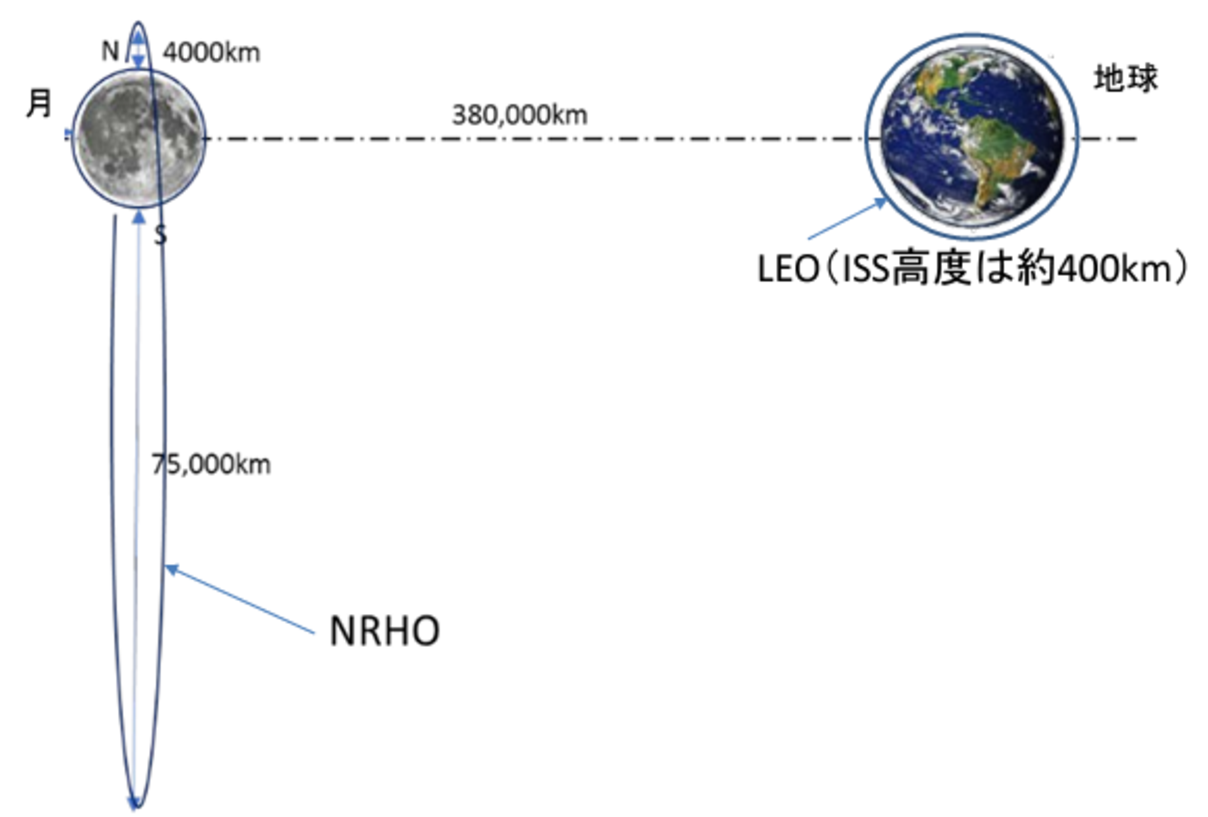
\includegraphics[width=0.7\textheight]{img/artemis_moon_station_orbit.pdf}
    \caption{アルテミス計画におけるステーションの投入予定軌道}
    \label{fig:artemis_moon_station_orbit}
    \begin{minipage}{\textwidth}
        \centering
        \vspace{3mm}
        \fontsize{10pt}{12pt}\selectfont
        参考文献\cite{kiban_dai48}9ページより抜粋
    \end{minipage}
\end{figure}

アルテミス5ではさらにローバーによる月面探査などが計画されている. 
アルテミス計画は当初の計画よりも遅延が発生しているものの, 
アルテミス1は2022年11月16日に打ち上げられ, 25日後の12月11日に地球に帰還した. 
アルテミス2は2026年4月に, アルテミス3は2027年中旬に予定されている. 
アルテミス計画ではNASAのみならず, 
宇宙航空研究開発機構(Japan Aerospace Exploration Agency : JAXA), 
欧州宇宙機関(European Space Agency : ESA), 
カナダ宇宙庁(Canadian Space Agency : CSA)も主要な開発に参加している. 
\cite{jaxa2021}

\subsection{アルテミス計画以外の月探査計画}
\label{section:アルテミス計画以外の月探査計画}

International Lunar Research Station(ILRS)は, 
中国国家航天局(CNSA)とロシア連邦宇宙局(ROSCOMOS)が主導する
2024年9月時点で13カ国が参加している月面基地プロジェクトであり, 
月表面/月軌道においてさまざまな研究や技術実証が計画されている\cite{ilrs}. 
プロジェクトは主に以下の3つの段階に分けられている. 
2021年~2025の調査フェーズでは, ILRSの初期段階として 
月面の詳細な調査が行われ, ILRSの設計と建設候補地の選定, 
月面での高精度かつ安全な軟着陸を実現するための技術検証などが行われる. 
2026年~2035年の建設フェーズでは, さらにステージ1と2に段階を分けて計画が進められる. 
ステージ1ではILRSの指令センターにおける技術検証, 月サンプルの回収, 
大量貨物の輸送と高精度で安全な軟着陸の実現が目指され, ILRSの共同運用が正式に開始される. 
ステージ2ではILRSの包括的な構築が進められ, エネルギー供給, 通信, 輸送サービスを
はじめとする軌道上および月面施設の整備が完了し, ILRSが完成する. 
2036年以降の利用フェーズでは, ILRSは科学研究や探査, 技術検証のための拠点として活用され, 
有人月面ミッションの支援や, 必要に応じた施設の拡張や保守も行われる予定である. 

\subsection{アルテミス計画以外の火星探査計画}
\label{section:アルテミス計画以外の火星探査計画}
アルテミス計画以外にも火星探査計画は各国宇宙機関により計画・実施されている図\ref{fig:mars_explorations}
NASAのPerseveranceやESAとロシアの国営宇宙公社ロスコスモス(State Space Corporation: ROSCOSMOS)のExoMarsなどが進行中で, 
サンプルリターンや地震観測, 生命探査が行われている. 
また中国の「天問1号」も火星の地質と水の痕跡を調査中である. 
火星とその衛星であるフォボスとダイモスの探査計画は, 火星の地質や生命の痕跡調査, 
衛星の起源解明, 資源利用, そして人類の宇宙活動の基盤構築を目的としている. 
フォボスに関しては, JAXAの「MMXミッション」が注目されている. 
この計画では, フォボスに対しサンプルリターンを行い, 衛星の起源を探る予定である. 
またフォボスは将来的に火星有人探査の中継拠点となる可能性もある. 
一方ダイモスは火星衛星探査計画(Martian Moons eXploration : MMX)の
フライバイ観測でデータが収集され, フォボスとの比較が行われる予定である. 

\begin{figure}[tbh]
    \centering
    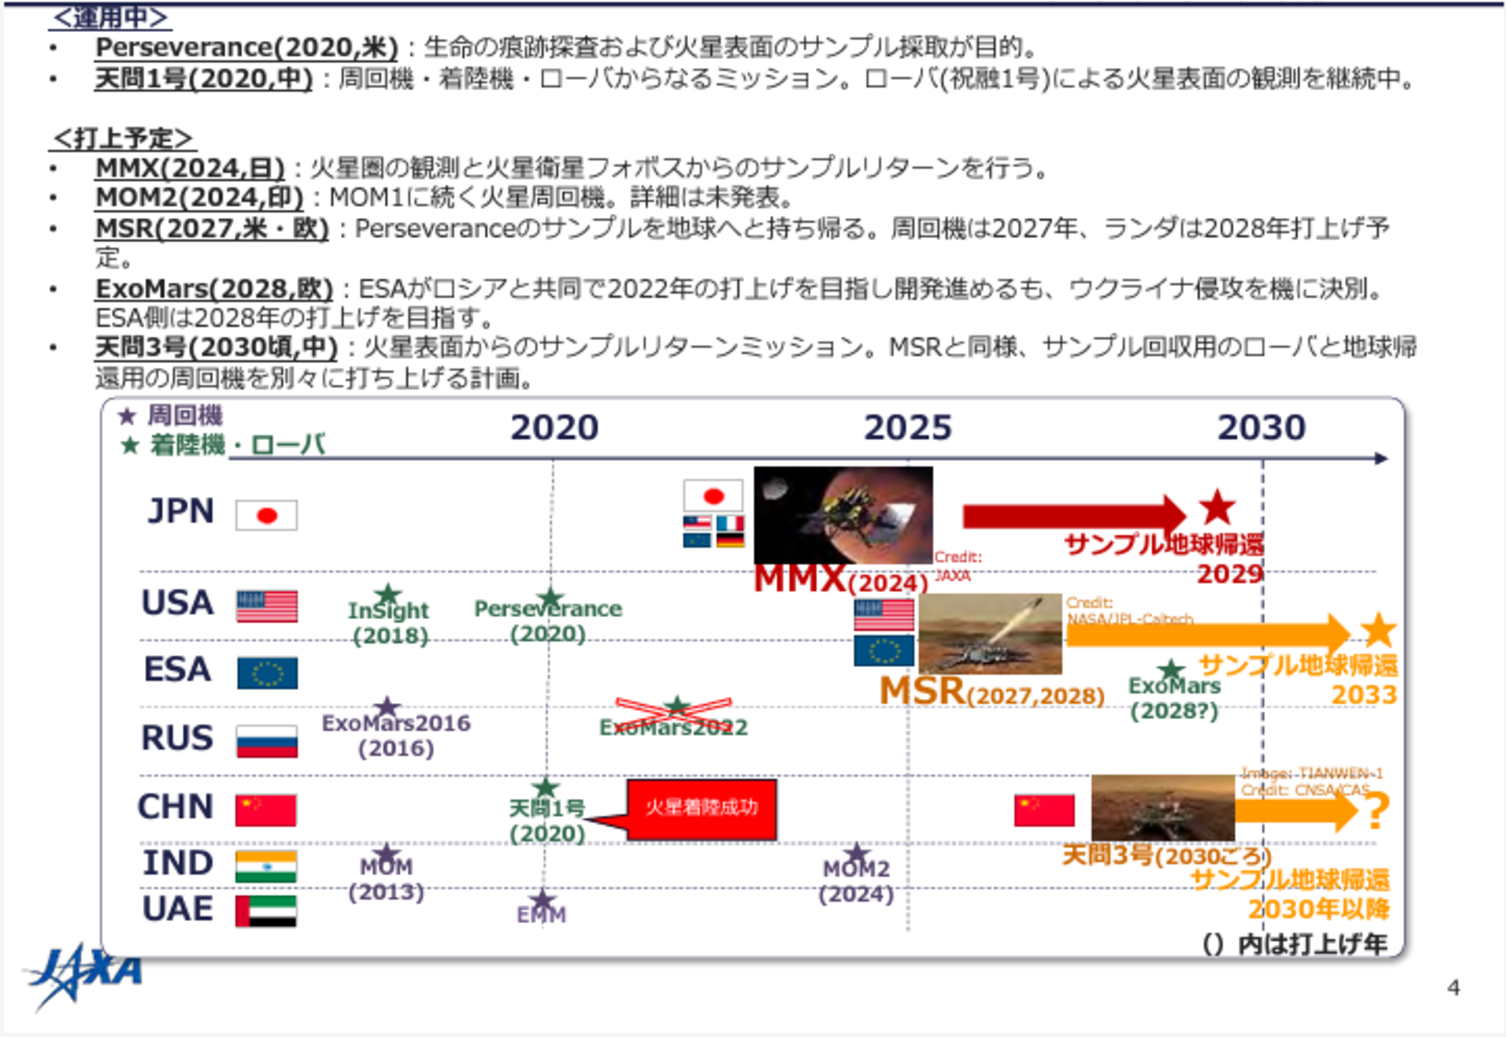
\includegraphics[width=0.7\textheight]{img/mars_explorations.pdf}
    \caption{各国の火星探査計画}
    \label{fig:mars_explorations}
    \begin{minipage}{\textwidth}
        \centering
        参考文献\cite{isas2023}4ページより抜粋
    \end{minipage}
\end{figure}

\subsection{民間事業者の宇宙事業への参画}
\label{section:民間事業者の宇宙事業への参画}
当初は軍事・政府関係の需要が中心であった宇宙開発は近年特に民間事業者の参画が進んでおり,
幅広い用途の宇宙開発が進められている. 
2022年時点での世界の宇宙産業規模は54兆円, さらに2040年までに140兆円規模に拡大すると
予想されている\cite{経産省2024}. また日本国内でも市場規模は約4兆円であり, 政府は2030年代早期の倍増(約8兆円)を目指している. 
打ち上げ事業では米国のSpaceXを筆頭に打ち上げ回数が増加しており, 
図\ref{fig:number_satellite_launched}のように2022年には米国の民間事業者だけで世界全体の打ち上げ回数の
約42\%を占めた. SpaceXの独占的な状態が続いてはいるものの, 各国の事業者も開発を続けている. 
\begin{figure}[tbh]
    \centering
    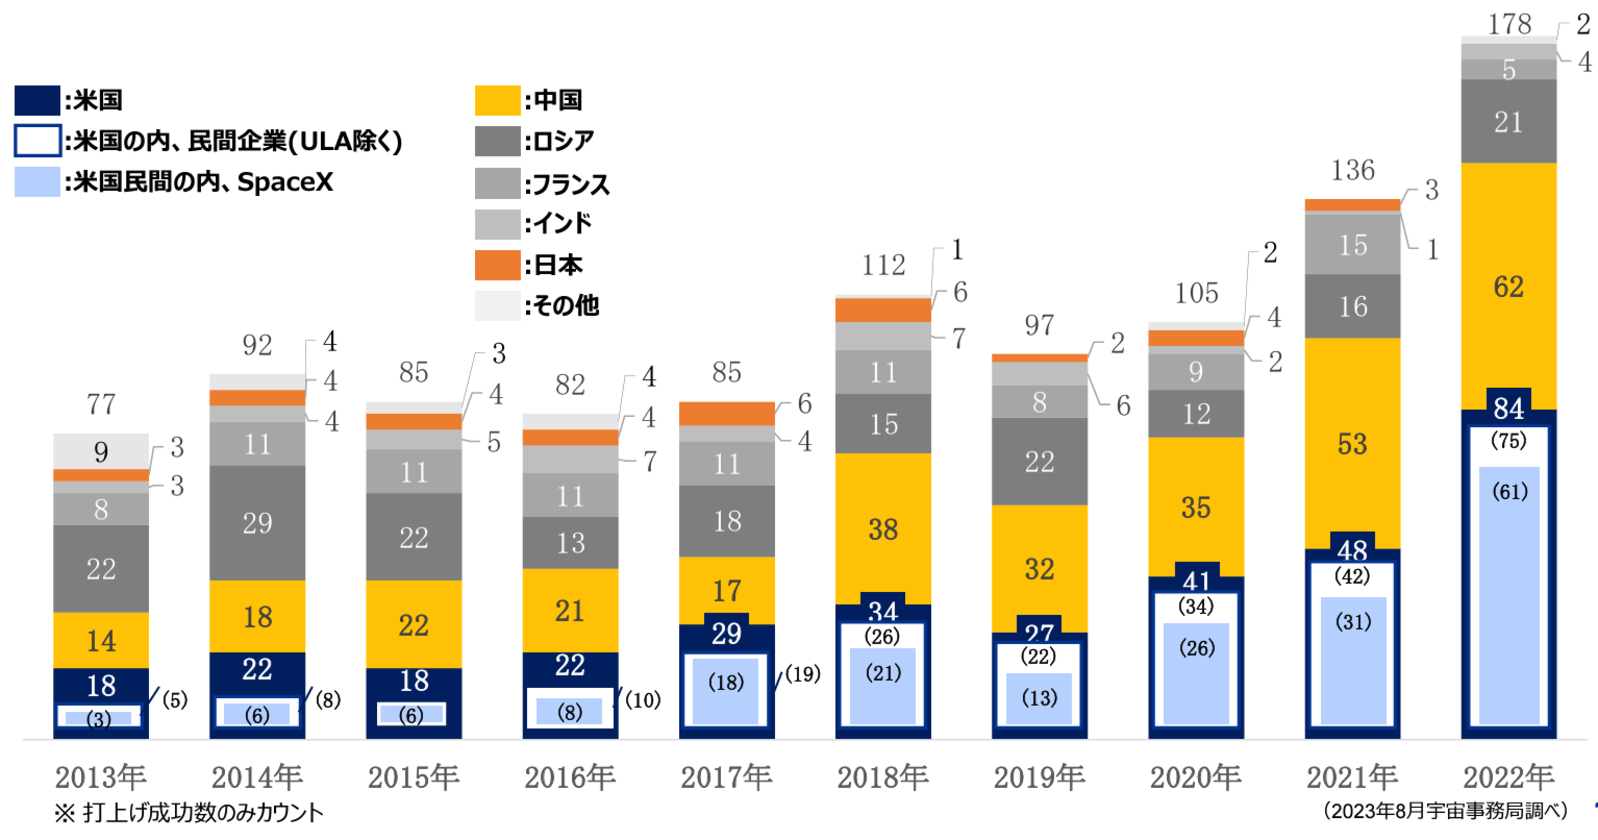
\includegraphics[width=0.7\textheight]{img/number_satellite_launched.pdf}
    \caption{世界のロケット打ち上げ数の推移}
    \label{fig:number_satellite_launched}
    \begin{minipage}{\textwidth}
        \centering
        \vspace{3mm}
        \fontsize{10pt}{12pt}\selectfont
        参考文献\cite{内閣府2023}10ページより抜粋
    \end{minipage}
\end{figure}


\section{宇宙通信におけるインターネット技術の適用可能性}
\label{section:宇宙通信におけるインターネット技術の適用性}
これらの宇宙開発計画に伴い,  月・火星の地表及びその近傍の空間に多くの人や宇宙機, その他機材が存在するようになり, 
天体内・天体間での通信需要が大きくなることが予想される.  
従来までの宇宙ミッションにおいて宇宙のノードと地球との通信は,  地球上にある各国の大型アンテナを利用し,  一対一の通信を行っていた. 
しかしこのような計画でノードの数が増加する場合, 通信ニーズに対応するためには宇宙にも多対多のノードで通信が可能な宇宙インターネットが必要となる.  
これに向け, 既存のインターネットの技術を宇宙インターネットに向け改良し活用することが検討されているが, 
当然ながら宇宙環境は地球とは環境が大きく異なり, 特に以下の部分に関して考慮が必要となる. 

\section{通信における宇宙の環境}
\label{section:通信における宇宙の環境}
宇宙環境は地球環境とは多くの点において異なるが, 
通信やネットワークに関しては\ref{section:大きな遅延のある通信環境}項や
\ref{section:ネットワークトポロジーの変動と間欠的接続}項のような違いが
重要となる. 


\subsection{大きな遅延のある通信環境}
\label{section:大きな遅延のある通信環境}
宇宙での通信は既存のインターネットにおける通信の遅延に比較して非常に大きい. 
東京-ニューヨーク間であれば, 伝搬遅延のみを考慮した場合, 片道50ms以内で通信が可能である一方, 宇宙における通信の際には地球月間でも片道1. 3秒, 
地球火星間では太陽に対する2天体の公転の状況によって変動するが最大20分程度の遅延が想定されている. 
End-to-EndでTCPを用いた通信を行う際には,  3-way-handshakeなどを含めこれらの天体間を複数回往復する通信を行う必要があり,  
遅延はさらに大きな時間になる.  
\cite{McBrayer2022}
また火星の衛星フォボスとダイモスについては, 
火星地表との平均距離がフォボスで9378km, ダイモスが23459kmとなっているため, 
光速を313000km/sと仮定すると, それぞれ0.030秒, 0.075秒程度未満の通信遅延が発生する. 


\subsection{ネットワークトポロジーの変動と間欠的接続}
\label{section:ネットワークトポロジーの変動と間欠的接続}
宇宙のインターネットにおいて, ネットワークを構成するノードには多くの宇宙機が含まれている. 
これらのノードは当然ながら宇宙空間での位置が常に変化しており, 
 天体の影に入るなどで断絶が頻繁に起こる.  

\section{Delay and Disruption Tolerant Networking(DTN)}
これらの宇宙環境におけるインターネットのコンセプトとして, Delay and Disruption Tolerant Networking(DTN)が
が構想されている. DTNの中心となる技術の一つにRFC9171\cite{rfc9171}で標準化されたBundle Protocol(BP)があり,  
BPでは通信されるデータはBundleという可変長のデータとして転送される.  
中間ノードでは経路上の次のノードへ転送可能なタイミングまでBundleを蓄積することが可能になっているため,  
End-to-Endの通信疎通性が確保できていない場合でも,  この蓄積による転送を行うことにより断絶に強い通信ができる. 
またトランスポートレイヤにUDPなどのプロトコルを用いることで,  比較的遅延を抑えて通信することもできる. \cite{bundle_protocol_architecture}

% \subsection{通信機会の非対称性}
% \label{subsection:通信機会の非対称性}

\begin{figure}[tbh]
    \centering
    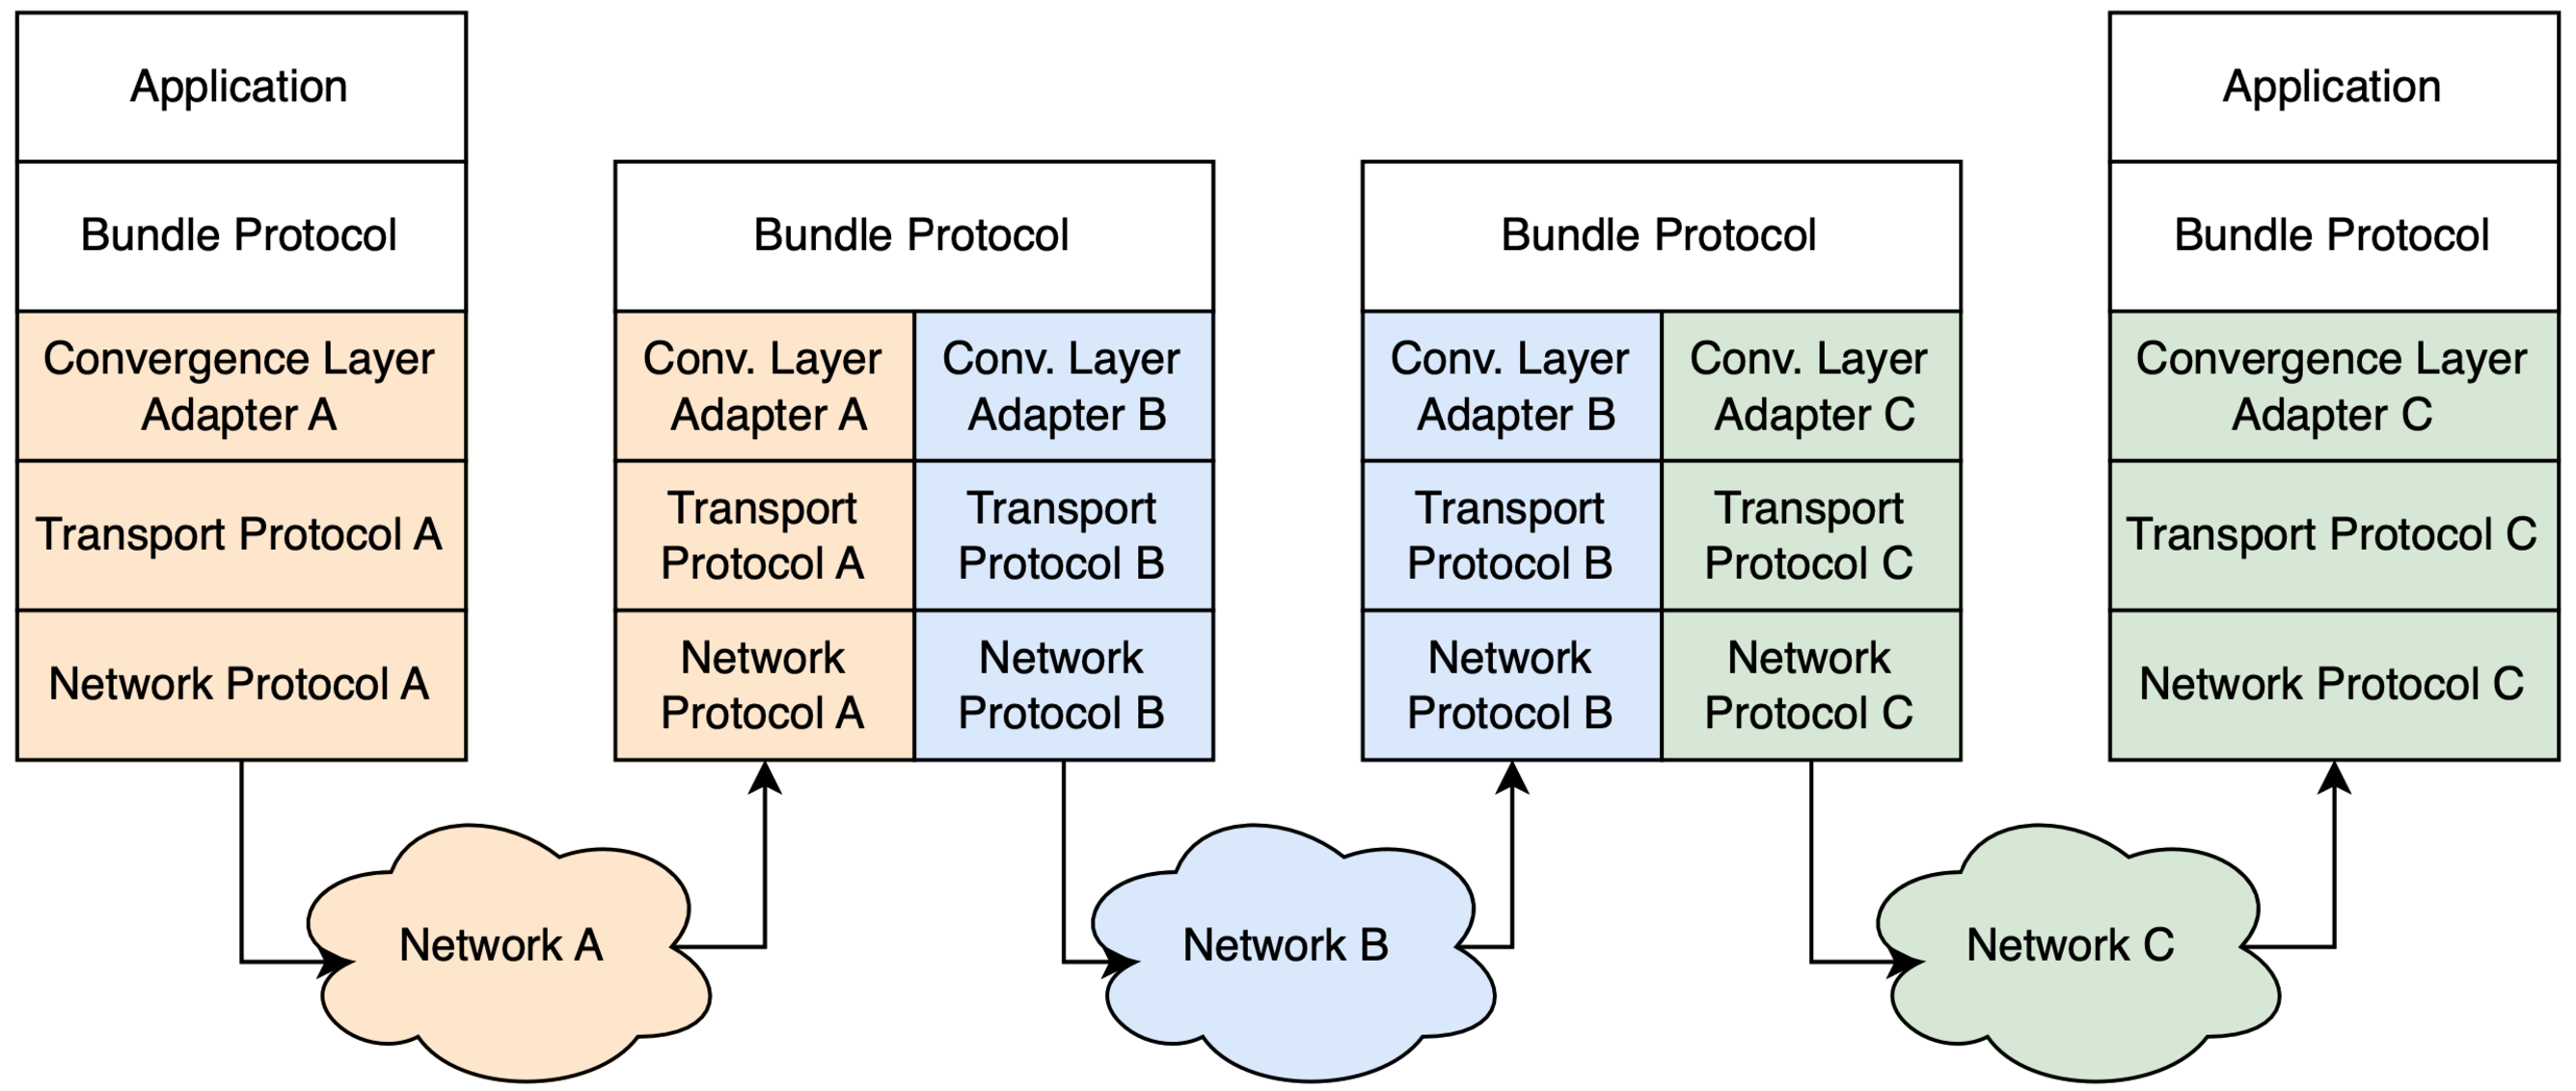
\includegraphics[width=0.7\textheight]{img/dtnprotocolstack.pdf}
    \caption{DTNを搭載したノード間のみでの通信}
    \label{fig:dtnprotocolstack}
    \begin{minipage}{\textwidth}
        \raggedright
        \vspace{3mm}
        \fontsize{10.5pt}{12pt}\selectfont
        参考文献\cite{bundle_protocol_architecture}Figure1をもとに作成. 
        図中のConvergence Layer(CL)については
        \ref{section:Convergence LayerとLTP}項で説明する.
    \end{minipage}
\end{figure}

\subsection{宇宙におけるDTN}
DTNは当初惑星間インターネットのアーキテクチャのコンセプトとして構想された. しかしRFC 4838\cite{rfc4838}において, 
Delay Tolerant Networkingという言葉を使用した頃から, 地上無線ネットワークへの適用も構想されるようになった. 
これらの環境と宇宙環境でのDTNの大きな違いとして, 通信機会のタイミングが挙げられる. 
\ref{chap:cgr_in_dtn}章でも述べるが, 
宇宙環境でのDTNにおいてはノード間の通信機会は全て予測可能なものである一方, 
地上無線ネットワークでの通信機会は予測が難しいものであり, そのためルーティングの手法なども異なる. 
本研究では宇宙のインターネットにおけるルーティング手法に注目しているため, 以後は地上無線ネットワークにおけるDTNではなく, 
宇宙インターネットで用いるDTNについて議論する. 

\subsection{Bundle Protocol}
\label{subsection:Bundle Protocol}
上記でも述べたBPは, DTNにおける主要な通信技術で遅延・断絶が起きやすい環境でデータを確実に伝送するために設計された. 
このBundleは,  送信元から目的地までの途中で複数の中継を経ても, 全体としてデータを確実に届けるためのものである.  
また, このプロトコルは「ストア&フォワード」方式を利用しており,  各中継ノードが受け取ったBundleを一時的に保存し,  
次のノードと通信できるタイミングが来るまで待機する.  これにより, 通信が一時的に途絶えてもデータが失われることなく,  次のノードへと送信される. 

\subsection{IPN address}
\label{subsection:IPN address}
IPNアドレス(Interplanetary Networking Address)は, DTN環境で使用されるアドレス形式で, 
宇宙通信のためのネットワーク識別とエンドポイントの識別を可能にするものである. 従来のインターネットプロトコルアドレス(IPアドレス)は, 
リアルタイムでの通信や短い遅延を前提とした設計であるため, 宇宙空間における遅延や断絶が発生する環境では適切に機能しない. 
DTNのアーキテクチャは, これらの遅延や断絶を前提としており, IPネットワークとは異なる方法でデータを伝送するため, 
IPNアドレスが必要とされている.  さらに,  IPNアドレスは地上のインターネットや宇宙のネットワークなど, 
異なるアドレッシングスキームを持つネットワークの統合する役割としても機能する. 
IPNアドレスは「ipn:ノード番号. サービス番号」という形式で記述され, これにより特定の宇宙船や装置が個別に識別される.  

\subsection{Convergence LayerとLTP}
\label{section:Convergence LayerとLTP}
DTNでは多様なプロトコルがトランスポートレイヤ以下の層で使用することを想定しており,  
図\ref{fig:dtnprotocolstack}中のConvergence Layerは
それらの違いを吸収することを目的としている.  Convergence Layer Protocol(CLP)としては,  
利用する下位レイヤプロトコルにより, 

\begin{itemize}
    \item TCP-based CLP (TCPCL)
    \item User Datagram Protocol (UDP)-based CLP (UDPCL)
    \item Saratoga CLP
    \item Licklider Transmission Protocol (LTP)-based CLP (LTPCL)
\end{itemize}

などがある. 
LTP\cite{rfc5326}はコンバージェンスレイヤのプロトコルの一つであり,  再送制御の機能も実装している. 
LTPをコンバージェンスレイヤに用いる場合,  トランスポートレイヤにUDPを用いることがあるほか,  
宇宙での通信においてLTPが直接リンク層にアクセスすることも想定されている. 

\subsection{既存のDTN実装}
\label{section:既存のDTN実装}
既にいくつかの研究機関などによりDTN技術を実装したソフトウェアがリリースされている.  いくつかの例を以下に示す.  
\begin{itemize}
    \item Interplanetary Overlay Network DTN(ION-DTN): NASA/JPL
    \item HDTN : NASA/Glenn research center
    \item DTN ME : Marshall Space Flight center
    \item \textmu D3TN : D3TN GmbH
    \item IONe : Experimental ION Scott Burleigh United States 
    \item DTN7/Go : University of Marburg German
\end{itemize}
これらのDTNソフトウェアは,  基本的に通信内容からBundleへのエンコード・デコード,  
中間ノードでのBundleのままでの蓄積転送を可能にしているが,  
Convergence Layerが対応しているトランスポートレイヤプロトコルの種類などの点で異なる. 
これらの実装についての比較についてを表\ref{table:chart_dtn_implementations}に示す. 

\begin{table}[tbh]
    \centering
    \caption{DTN実装とその機能の比較}
    \begin{minipage}[t]{\textwidth}
        \centering
        \fontsize{10.5pt}{12pt}\selectfont
        参考文献\cite{dtn_implementations}figure1より抜粋
        \vspace{3mm}
    \end{minipage}
    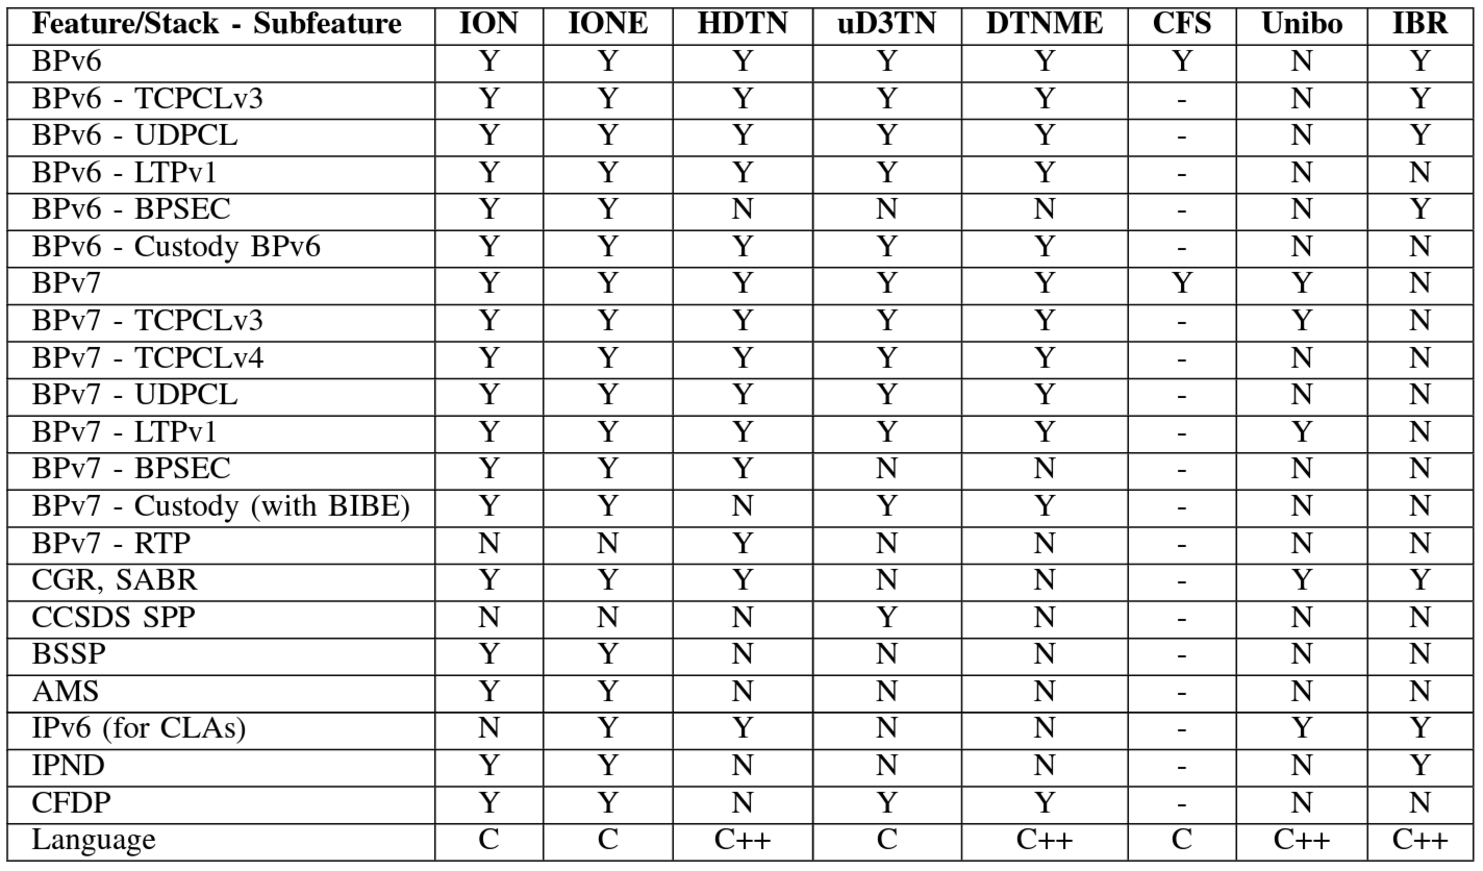
\includegraphics[width=0.7\textheight]{img/chart_dtn_implementations.pdf}
    \label{table:chart_dtn_implementations}
\end{table}